\documentclass[paper=letter, fontsize=12pt]{article}

\usepackage[english]{babel} % English language/hyphenation
\usepackage{amsmath,amsfonts,amsthm} % Math packages
\usepackage[section]{placeins}  % prevent figures / eqns / tables 
                                % from slipping out of section.
\usepackage{sectsty} % Allows customizing section commands
\allsectionsfont{\centering \normalfont\scshape} % Make all sections centered, 
                                                 % the default font and small 
                                                 % caps 

\usepackage{fancyhdr} % Custom headers and footers

% algorithms
\usepackage{algorithm}
\usepackage[compatible]{algpseudocode}

\usepackage{ragged2e} % Text alignment
\usepackage[margin=1in]{geometry} % 1 inch margins
\usepackage{tikz} % Not always necessary, but allows very customizable 
                  % figures / object placement
\usepackage{enumitem} % get more out of enumerate

% begin additional packages
\usepackage{hyperref}
\usepackage{blindtext}
% end additional packages

% Header and Footers
\pagestyle{fancyplain} % Makes all pages in the document conform to the custom 
                       % headers and footers
\fancyhead{} % No page header
\fancyfoot[L]{} % Empty left footer
\fancyfoot[C]{} % Empty center footer
\fancyfoot[R]{\thepage} % Page numbering for right footer
\renewcommand{\headrulewidth}{0pt} % Remove header underlines
\renewcommand{\footrulewidth}{0pt} % Remove footer underlines
\setlength{\headheight}{13.6pt} % Customize the height of the header

% Number all figs, eqns, and tables within the section
\numberwithin{equation}{section} % Number equations within sections 
\numberwithin{figure}{section} % Number figures within sections 
\numberwithin{table}{section} % Number tables within sections 

\setlength\parindent{4pt} % 4pt indentation for paragraphs
\setlength{\parskip}{\baselineskip} % adds some spacing in between paragraphs

\newcommand{\horrule}[1]{\rule{\linewidth}{#1}} % Create horizontal rule command
                                                % with 1 argument of height
\newcommand{\fancyline}{\\ \horrule{0.5pt} \vspace{0.1cm}} % fancy line to put
                                                           % under questions

%  Some commands for algorithm environments                                            
\renewcommand{\algorithmicrequire}{\textbf{Input:}}
\renewcommand{\algorithmicensure}{\textbf{Output:}}
\renewcommand{\algorithmicforall}{\textbf{for each}}
\newcommand{\algorithmiccontinue}{\textbf{continue}}
\algloopdefx{RETURN}[1][]{\textbf{return} #1}

% useful math shortcuts
\newcommand{\lagr}[1]{\mathcal{L}\left( #1 \right)}
\newcommand{\expval}[1]{E\left[#1\right]}
\newcommand{\var}[1]{\text{var}\left(#1\right)}
\renewcommand{\det}[1]{\text{det}\left(#1\right)}
\newcommand{\diag}[1]{\text{diag}\left[#1\right]}

% begin additional definitions and commands

% end additional definitions and commands

%-------------------------------------------------------------------------------
%	TITLE SECTION
%-------------------------------------------------------------------------------

\title{	
\normalfont \normalsize 
\textsc{RICE UNIVERSITY COMP540} \\ [25pt]
\horrule{0.5pt} \\[0.4cm] % Thin top horizontal rule
\huge deton8: Detector of Nuclei \\ % The assignment title
\horrule{2pt} \\[0.5cm] % Thick bottom horizontal rule
}

\author{Will LeVine \& Gabriel Vacaliuc}

\date{\normalsize\today}

\begin{document}

\maketitle

\begin{abstract}
    \blindtext
\end{abstract}

\newpage

\tableofcontents

\newpage


%-------------------------------------------------------------------------------
%   CONTENT
%-------------------------------------------------------------------------------

\section{Introduction}

Modern medical research generates an incredible amount of data that requires
significant time to be processed in some way.  Often some of this processing
involves tedious manual hand labeling of data, such as images, simulations, or
video.  To this end, it is desirable for medical research to develop automated
processes so as to allow trained professionals to focus on more challenging
problems than rote labeling.  An example of one of these problem ripe to be
solved is the labeling of microscopic cell nuclei in image data.  As such, the
2018 Data Science Bowl is focused on solving this problem, or at least
advancing the current state of the art.  We've included the corresponding
\href{https://www.kaggle.com/c/data-science-bowl-2018}{kaggle competition}'s
description below:

\begin{quote}
    \textbf{\large Spot Nuclei. Speed Cures.}

    Imagine speeding up research for almost every disease, from lung cancer and
    heart disease to rare disorders. The 2018 Data Science Bowl offers our most
    ambitious mission yet: create an algorithm to automate nucleus detection.

    We’ve all seen people suffer from diseases like cancer, heart disease,
    chronic obstructive pulmonary disease, Alzheimer’s, and diabetes. Many have
    seen their loved ones pass away. Think how many lives would be transformed
    if cures came faster.

    By automating nucleus detection, you could help unlock cures faster—from
    rare disorders to the common cold. Want a snapshot about the 2018 Data
    Science Bowl? \href{https://www.youtube.com/watch?v=eHwkfhmJexs}{View this
    video.}

    \textbf{\large Why nuclei?}

    Identifying the cells’ nuclei is the starting point for most analyses
    because most of the human body’s 30 trillion cells contain a nucleus full
    of DNA, the genetic code that programs each cell. Identifying nuclei allows
    researchers to identify each individual cell in a sample, and by measuring
    how cells react to various treatments, the researcher can understand the
    underlying biological processes at work.

    By participating, teams will work to automate the process of identifying
    nuclei, which will allow for more efficient drug testing, shortening the 10
    years it takes for each new drug to come to market.
    \href{https://datasciencebowl.com/2018dsbtutorial/}{Check out this video
    overview to find out more.}
\end{quote}

To begin understanding the task at hand, we're going to dive in and check out 
some images from the dataset.  We'll continue by explaining exactly what needs
to be done for a given image, followed by some commentary on the specific 
challenges of this competition.

\subsection{Dataset Examples}

The dataset contains an assortment of images of sizes ranging from (256, 256)
to (1024, 1024), however most images are on the smaller end.  Upon reading in
our images, we reshape them all to (256, 256) for simplicity.  Observe a sample
of our dataset in Figure \ref{fig:dsbowl18-grid}.

\begin{figure}
    \centering
    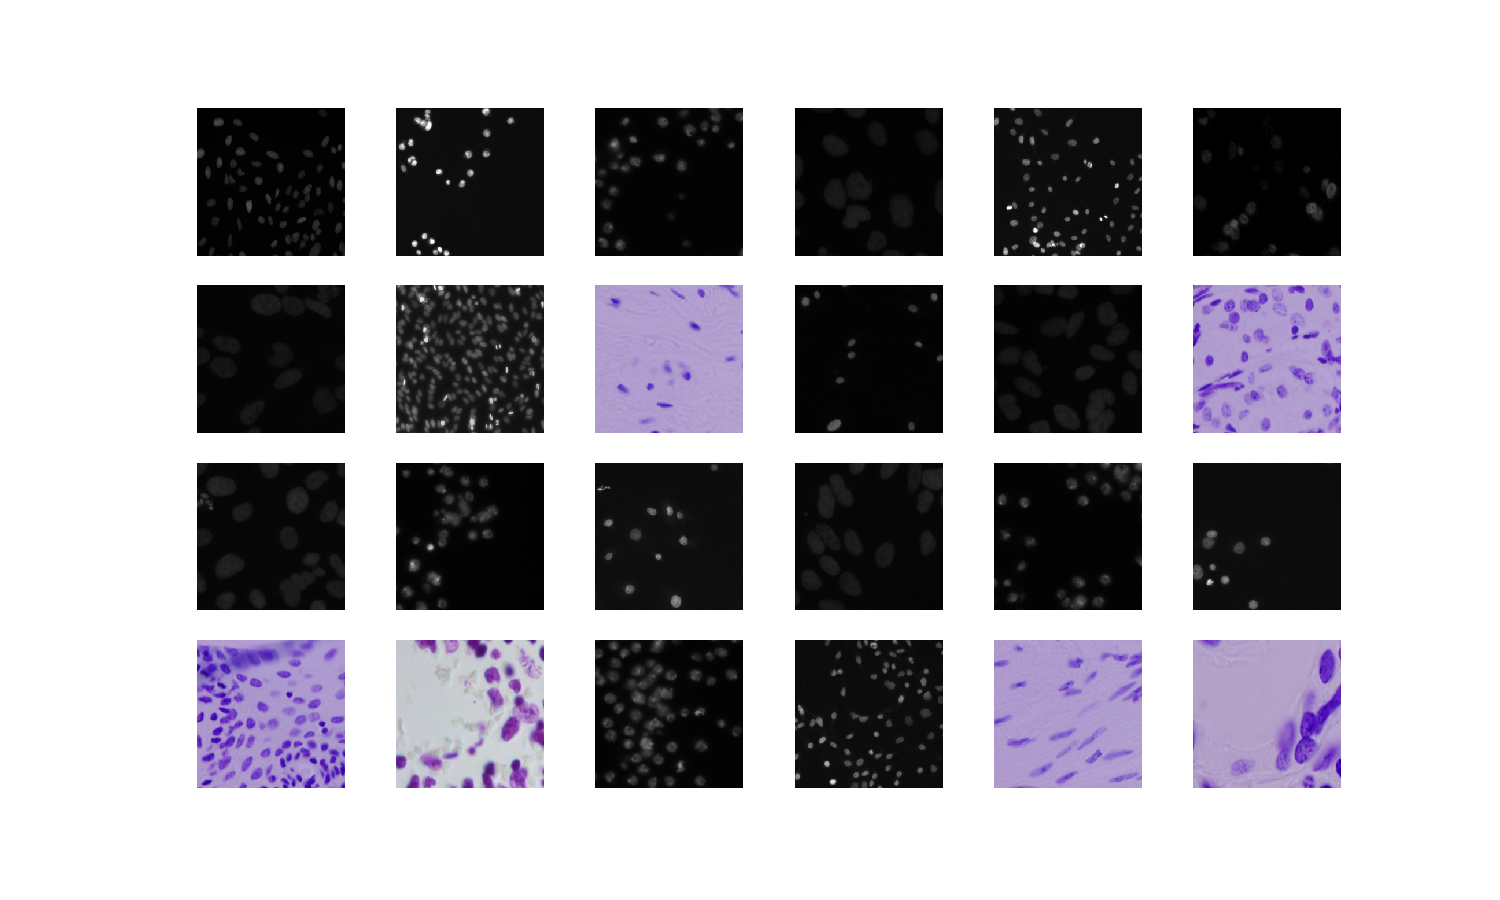
\includegraphics[width=\textwidth]{./figs/dsbowl18-imagegrid-4x6.png}
    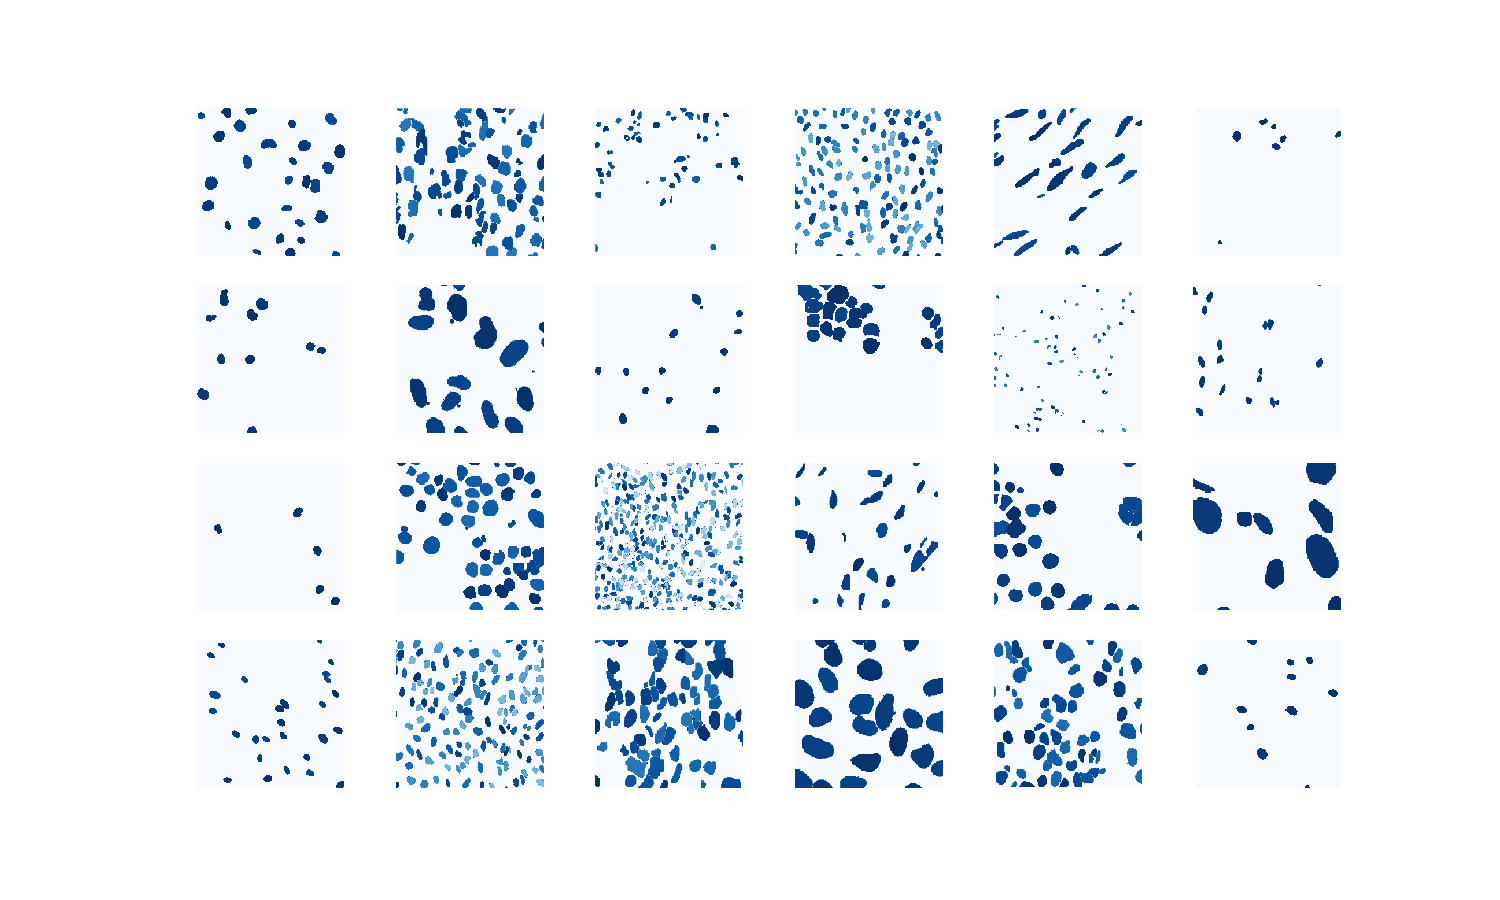
\includegraphics[width=\textwidth]{./figs/dsbowl18-imagegrid-masks-4x6.png}
    \caption{An assortment of images from our dataset.  All have been resized
    to 256 x 256.}
    \label{fig:dsbowl18-grid}
\end{figure}

\subsection{Formal Description of Task}

Here is a mathematical description of our task.  Given a dataset $\mathcal{D}$
composed of images, $x \in \mathbb{R}^{d}$, we'd like to learn a function $f :
\mathbb{R}^{d} \mapsto \mathbb{N}^{d}$ mapping each pixel in an input image to
a discrete nucleus label in the natural numbers.  It is key to understand that
this task is not binary classification, but rather a task of semantic
segmentation.  We wish to uniquely identify each nucleus in an image.

\subsection{Challenges}

While semantic segmentation is itself a very challenging task given any 
dataset, there are some key aspects of this competition which make our task
especially challenging.

\begin{enumerate}

    \item size of training dataset

        While the recent state of the art for semantic and instance
        segmentation has been dramatically advanced in recent years, MS-COCO,
        one of the most popular datasets for such a task contains more than
        330K images, with more than 200K of them
        labeled\footnote{http://cocodataset.org}.  In contrast, our dataset
        contains a mere 670 labeled images (along with many mislabelings)
        coupled with a 67 image validation set, and a 3019 image test set.

    \item composition of dataset

        As seen in Figure \ref{fig:dsbowl18-grid}, there exist a variety of
        image types.  More specifically, the dataset was constructed using 

\end{enumerate}

\subsection{Metric}

\section{Background}

\section{Methods}

\section{Results}

\section{Discussion}

\section{Conclusion}

\end{document}
